\documentclass[11pt, oneside]{article} 
\usepackage{geometry}
\geometry{letterpaper} 
\usepackage{graphicx}
	
\usepackage{amssymb}
\usepackage{amsmath}
\usepackage{parskip}
\usepackage{color}
\usepackage{hyperref}

\graphicspath{{/Users/telliott_admin/Tex/png/}}
% \begin{center} 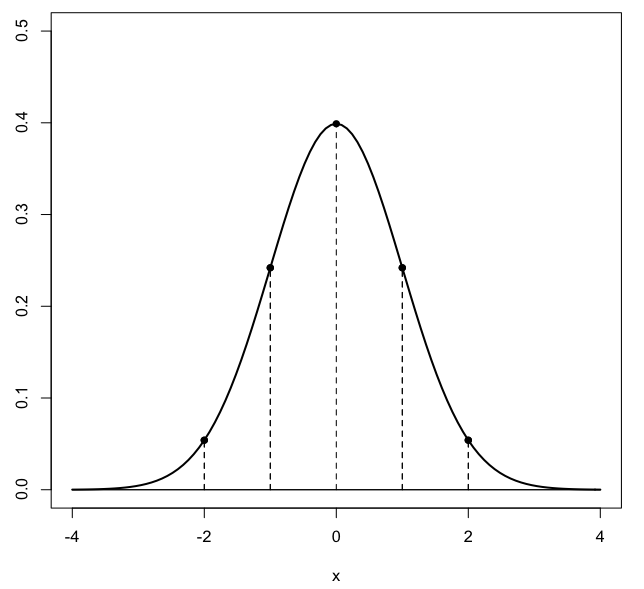
\includegraphics [scale=0.4] {gauss3.png} \end{center}

\title{Nahin Imaginary Tale Ch 2}
\date{}

\begin{document}
\maketitle
\Large
We start with a problem in analytical geometry:  to construct a line segment whose measure is the square root of a given line segment.
\begin{center} 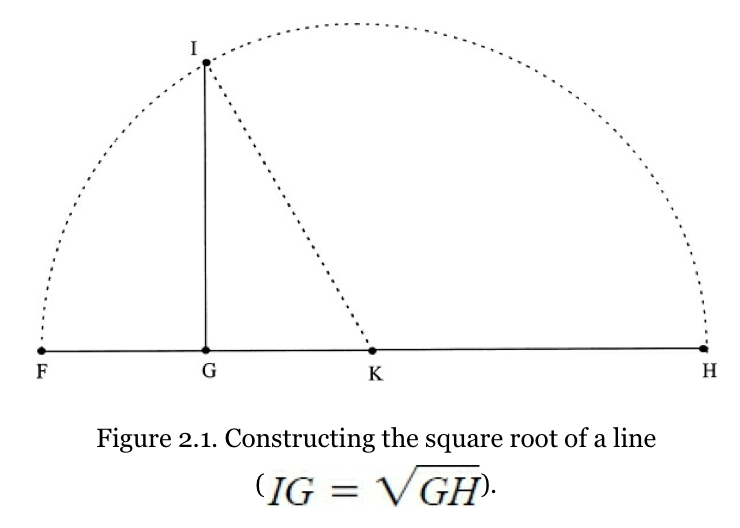
\includegraphics [scale=0.4] {Nahin_2_1.png} \end{center}

We are given $GH$.  Construct the rest of the diagram by extending $GH$ to $F$ by an as yet undetermined distance, find the midpoint, and then draw the circle.  Finally, extend the altitude $GI$.  

We will show that, for a particular value of $FG = x$, $GI$ is the square root of $GH$.

Let $R$ be the radius of the circle and $a$ be the altitude $GI$.

The base of the right triangle shown as $GK = R - x$.  Then Pythagoras says that:
\[ a^2 + (R  - x)^2 = R^2 \]
\[ a^2 = 2Rx - x^2 \]

In the particular case $x = 1$ (if $FG$ is unity), $a^2$ is equal to $2R - 1$, which is just $GH$.  $\square$

The next problem brings out another feature ( of the same diagram, with labels changed).  Draw $AP$.  Recall the famous theorem that $\triangle APC$ is a right triangle.

\begin{center} 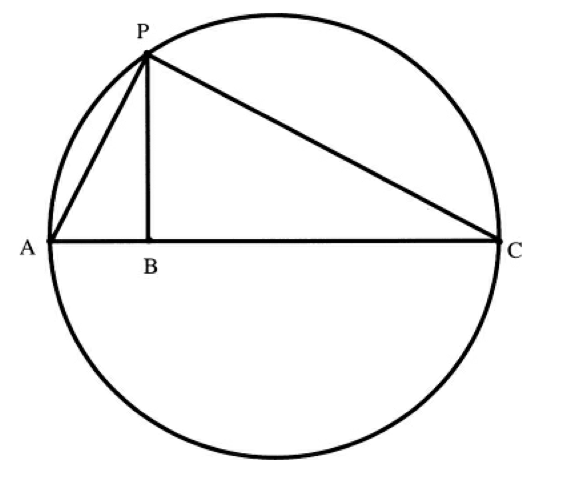
\includegraphics [scale=0.4] {Nahin_2_2.png} \end{center}

By similar triangles:
\[ \frac{AB}{BP} = \frac{BP}{BC} \]
\[ BP^2 = AB \cdot BC \]

This makes the solution to the previous problem quite obvious, substituting those labels we had
\[ a^2 = AB \cdot x \]
and we set $x = 1$ to get the solution.


\end{document}